\section{跨设备协同推理}
\label{sec:design-sys}
本节介绍 \sys-sys，即集成 \sys-PIM、通过软硬件协同设计实现高吞吐量的 AFD 系统；它旨在解决设备间数据同步与进度同步的开销问题。

\begin{figure}[t]
  \setlength{\abovecaptionskip}{2pt}
  \setlength{\belowcaptionskip}{-10pt}
  \centering
  \begin{minipage}[t]{\linewidth}
    \centering
    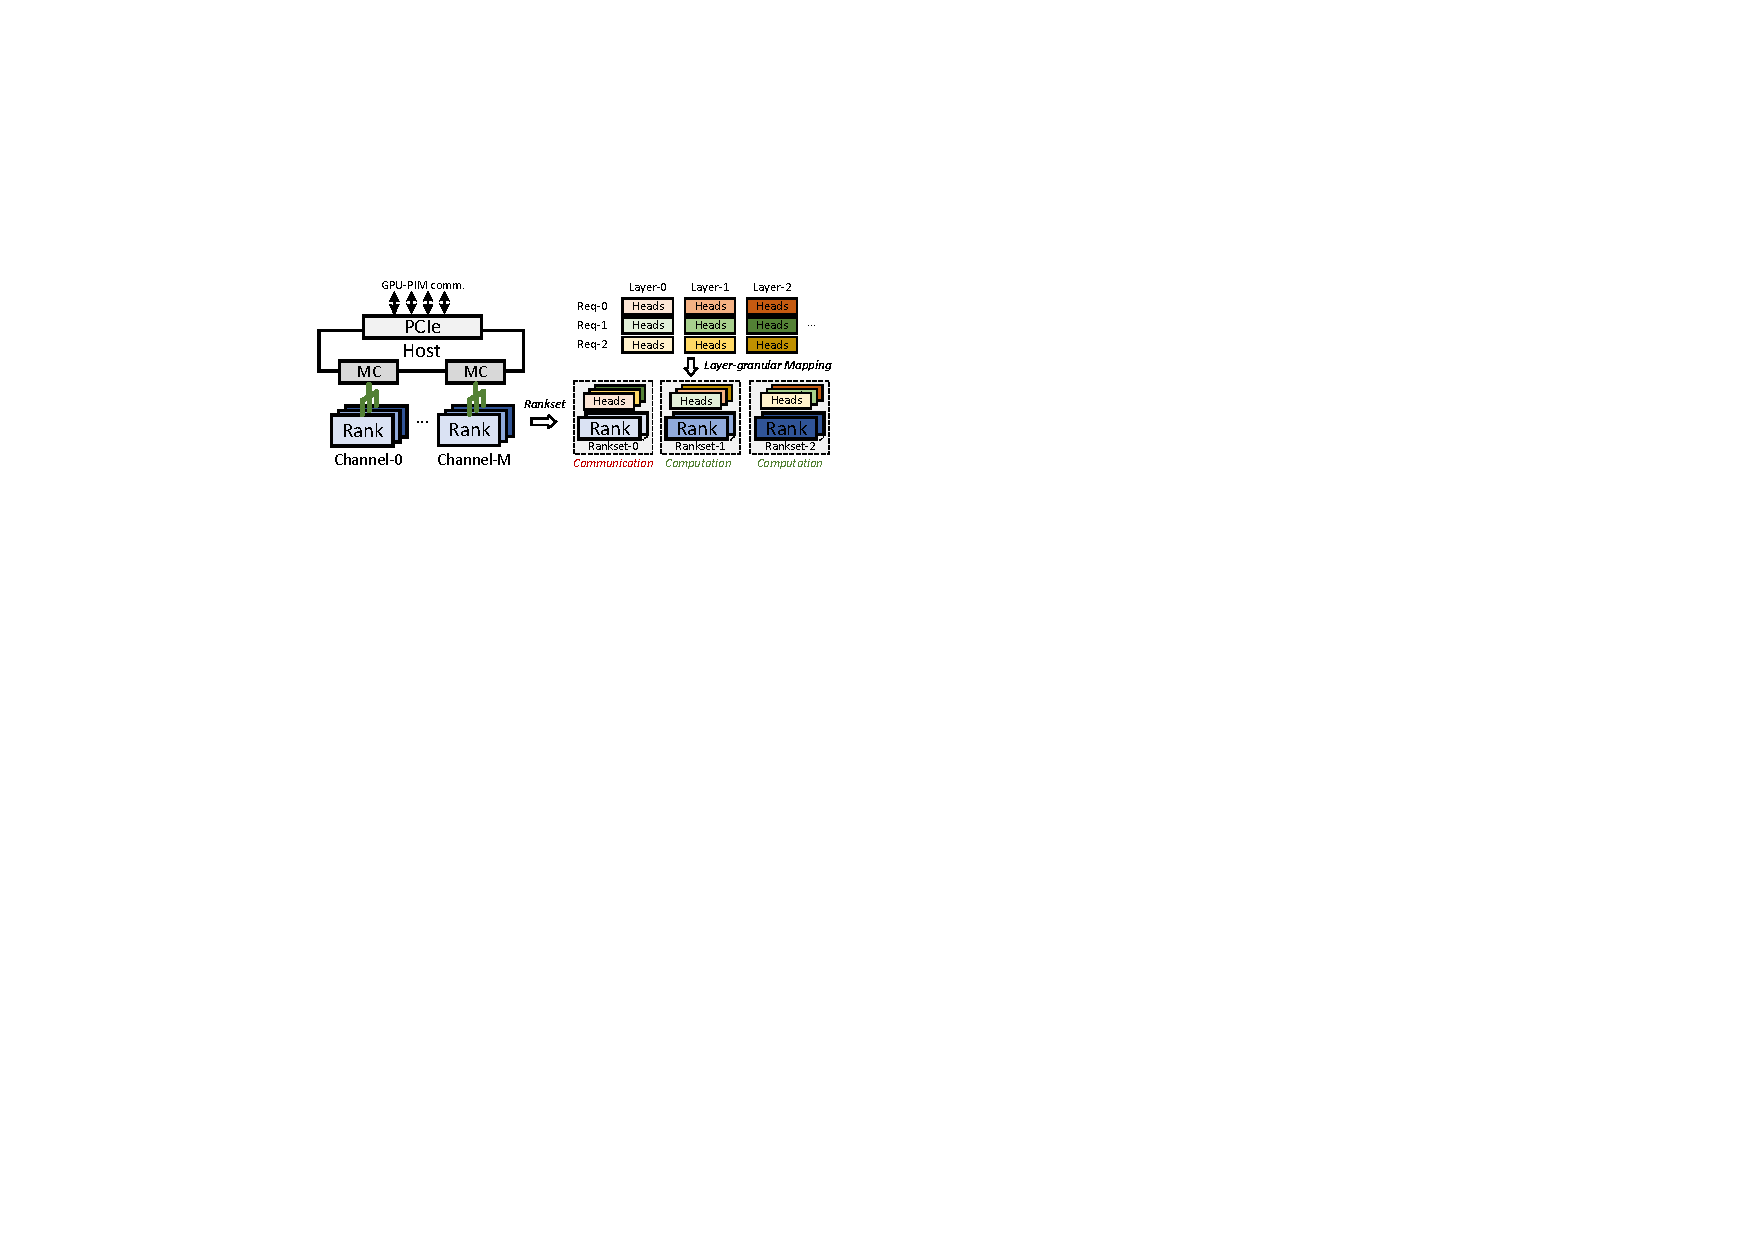
\includegraphics[width=\textwidth]{figs/design-rankset.pdf}
    \footnotesize
  \end{minipage}
  \caption{\textbf{以秩组粒度重叠通信与计算，隐藏数据传输开销。}}
  \label{fig:design-zigzag-rankset}
\end{figure}

\begin{figure*}[t]
  \setlength{\abovecaptionskip}{-1pt}
  \setlength{\belowcaptionskip}{-5pt}
  \centering
  \begin{minipage}[t]{0.9\linewidth}
    \centering
    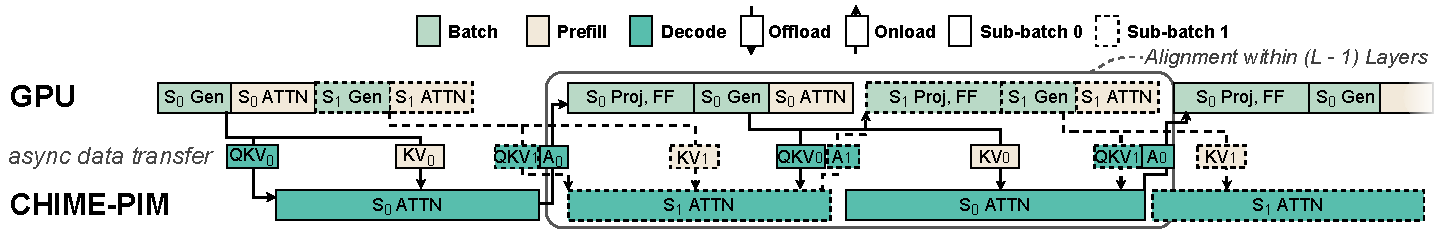
\includegraphics[width=\textwidth]{figs/design-zigzag.pdf}
    \footnotesize
  \end{minipage}
  \caption{\textbf{使用 \sys-sys 协调跨设备推理。}
  \textit{\sys 隐藏通信成本，并对齐跨设备并行执行。“ATTN”表示解码或预填充 Attention，“Gen”表示 QKV 生成，“Proj, FF”表示投影与前馈操作。}}
  \label{fig:design-compute-graph}
\end{figure*}

\subsection{秩组粒度通信--计算重叠}
\label{sec:design-sys-comm}
GPU 与 \sys-PIM 之间的数据同步包括传输以下数据：
(1) 预填充 K、V（与输入长度成正比）；
(2) 解码 QKV（每个请求一个 Token）；
(3) 解码 Attention 结果（每个请求一个 Token）。
理想情况下，采用子批次调度后可以异步传输这些数据，例如在执行一个子批次时发送另一个子批次的解码 QKV。
然而，GPU--PIM 数据通信与 \sys-PIM 上的 Attention 计算共享内存总线，这意味着通信会阻塞计算。
这种阻塞妨碍异步数据传输并带来不可忽略的开销，因为 PCIe 带宽~\cite{pci2025pci}可能比 \sys-PIM 的带宽低若干数量级（表~\ref{tab:simulator}）。

我们发现，挑战源于粒度过粗，即把所有 Rank 视作整体，只能统一执行通信或计算。
解决该问题的关键，是找到可独立、并发执行通信与计算的最细粒度。

\myparagraph{秩组粒度通信--计算重叠。}
我们的关键观察是：\emph{由于共享内存总线，在通信期间，一个通道内同一时刻只能访问一个 Rank，而其他 Rank 保持空闲。}
这促使我们提出\emph{秩组（rankset）}：它由每个通道中的一个 Rank 构成，是独立通信与计算的基本粒度。
因此，一个秩组是能够充分利用所有通道的最小 Rank 集合。
如图~\ref{fig:design-zigzag-rankset} 所示，每个通道包含三个 Rank，从而形成三个秩组。
当一个秩组进行通信时，其他秩组可以独立计算而不被阻塞，因此在通信期间仍可保留 $2/3$ 的计算能力。

此外，我们利用\emph{各层 KV cache 大小相同}这一特征，实现\emph{秩组粒度负载均衡}。
具体而言，我们以层为粒度、采用交错方式存储每个请求的 KV cache。
这样可均衡各秩组的数据传输负载，避免传输数据最多的秩组拖慢总体进度。

\subsection{对齐预测调度}
\label{sec:sys-scheduler}
为避免两个设备间并行操作进行进度同步所产生的空闲气泡，\sys 调度器的关键在于正确选择请求组成子批次，\emph{使两个设备上并行操作的执行延迟对齐}。
然而，LLM 的自回归特性使这种对齐颇具挑战，因为执行延迟会随已处理 Token 数、批大小等因素变化。
以往 AFD 系统未能实现这一目标：
对于基于 HBM-PIM 的 AFD 系统~\cite{park2024attacc,heo2024neupims}，PIM 侧延迟可能始终小于 GPU 侧（如图~\ref{fig:intro-motiv}-b 所示）；
基于 CPU 的 AFD 系统~\cite{jiang2024neo}则未在调度时对各操作执行延迟建模。
此外，CPU 侧计算时间可能受其他 CPU 应用干扰，因而缺乏可预测性~\cite{christina2013paragon,liu2024jiagu,lo2015heracles}。

\myparagraph{性能建模的机会。}
为解决这一挑战，\sys 提出\emph{对齐预测调度}，其关键特征是对两个设备的执行延迟进行建模与预测，以帮助对齐并行执行延迟。
利用这一能力，调度器选择请求组成子批次，使其在两个设备上的预测延迟对齐，如图~\ref{fig:design-compute-graph} 所示。
\sys 利用以下机会实现性能可预测性。
第一，\sys-PIM 上的执行\emph{不受干扰}。
第二，影响批次性能的因素（例如批大小、已处理 Token 数等）均可预先获得。
第三，大量既有工作已经探索 GPU 执行预测方法~\cite{cui2021abacus,gujarati2020clockwork,yang2022infless}。

\subsection{调度实现细节}
\myparagraph{模型特征。}
\sys 使用以下参数描述子批次 $i$：
$c_{p_i}$，各预填充请求的 Chunk 大小列表；
$f_{p_i}$，各预填充请求已完成 Token 数列表；
$f_{d_i}$，各解码请求（在每个 Rank 上）已完成 Token 数列表。
两个子批次的延迟可建模如下：
\begin{align}
  \label{equ:obj_1} &T_{{\rm GPU}_{0}} = t_p(c_{p_0}, f_{p_0}) + t_{\rm batch}(c_{p_0}, f_{d_1}) \\
  \label{equ:obj_2} &T_{{\rm PIM}_{0}} = t_d(f_{d_0}) + t_{\rm comm}(f_{d_0}, c_{p_1}) \\
  \label{equ:obj_3} &T_{{\rm GPU}_{1}} = t_p(c_{p_1}, f_{p_1}) + t_{\rm batch}(c_{p_1}, f_{d_0}) \\
  \label{equ:obj_4} &T_{{\rm PIM}_{1}} = t_d(f_{d_1}) + t_{\rm comm}(f_{d_1}, c_{p_0})
\end{align}
式~\ref{equ:obj_1}、\ref{equ:obj_3} 表示 GPU 侧延迟，其中包含预填充 Attention 与批量 FC 操作延迟。
式~\ref{equ:obj_2}、\ref{equ:obj_4} 表示 Rank 粒度的 \sys-PIM 延迟，其中包含解码 Attention 延迟以及与之重叠的数据传输开销。

\myparagraph{调度策略。}
调度策略通过以下步骤选择请求组成子批次，使跨设备并行执行对齐：
\begin{enumerate}
  \item 向每个子批次加入一个预填充请求；如果没有预填充请求，则跳过此步骤。
  \item 每加入一个预填充请求（意味着 $T_{GPU}$ 增加），\sys 就向每个子批次加入 $N$ 个解码请求，并以负载均衡方式将其分配给各 Rank。随后，它预测每个子批次的 $T_{PIM}$ 与 $T_{GPU}$。若 $T_{PIM}<T_{GPU}$，则继续加入 $N$ 个解码请求，直至 $T_{PIM}>T_{GPU}$。
  \item 若仍有预填充请求，则重复步骤 (1)，直至 PIM 内存耗尽。当内存已满且气泡位于 PIM 侧时，对每个子批次最后一个预填充请求进行分块，动态调整 $T_{\rm GPU}$，使其尽可能接近另一个子批次的 $T_{\rm PIM}$。
\end{enumerate}

$N$ 越大，批次执行时间的调整粒度越粗，但越有利于在不同 Rank 之间实现请求负载均衡。
在我们的实现中，MHA 具有更多 Head，且可将这些 Head 均匀分配到各芯片，因此 MHA 的 $N$ 设为 1，而 GQA 的 $N$ 设为 16。

\myparagraph{模型选择。}
\label{sec:runtime-profiling}
下面介绍 \sys 如何对不同推理操作的执行延迟建模。
第一，为建模 $T_{\rm GPU}$，我们采用随机森林回归（RFR），因为它具有增量学习能力、低延迟和高精度三项优势。
大量既有工作已证明 RFR 能够高效预测执行延迟~\cite{liu2024jiagu,zhao2021gsight}；其他具有类似特征的模型也可使用。
第二，为建模 $T_{\rm PIM}$，考虑到 \sys-PIM 执行具有可预测性（即执行时间与计算或传输的 Token 数呈线性关系），我们可以使用简单快速的线性模型来建模 $t_{\rm comm}$ 和各 Rank 的 $t_d$。
总体 $t_d$ 由执行时间最长的 Rank 决定。
模型可由以下公式描述（以子批次 0 为例）：
\begin{align*}
  &T_{{\rm PIM}_{0}} = {\rm Linear}(\sum{f_{d_0}}, {\rm len}(f_{d_0}), \sum{c_{p_1}}) \\
  &T_{{\rm GPU}_{0}} = {\rm RFR}_p(c_{p_0}, f_{p_0}) + {\rm RFR}_{\rm batch}(\sum{c_{p_0}}, {\rm len}(f_{d_0}))
\end{align*}

\myparagraph{运行时性能剖析。}
\sys 采用运行时性能剖析，在推理过程中收集延迟及相应批次信息。
\sys 维护的数据集会随采集数据动态演化，并用于增量更新模型，从而适应执行环境的变化。
此外，我们按 8:2 划分收集到的 1000 个数据点，构成训练集和测试集，用于评估 \sys 调度器的预测模型。
实验结果表明，该模型具有良好的性能可预测性，预测相对误差低于 $\sim$1\%（中位数 $<0.5\%$）。
